%\documentclass[hidelinks,onecolumn]{emulateapj}
\documentclass[hidelinks]{article}
%\documentclass[hidelinks,preprint]{aastex6}
\usepackage{url}
\usepackage{multirow}
\usepackage{amsmath}
\usepackage{xcolor}
\usepackage{hyperref}
\usepackage{affils}
\usepackage{graphicx}
\usepackage{titlesec}
%\usepackage{affils}
\usepackage{authblk}
\usepackage{multirow}
%\citestyle{aa}


%here's a bunch of commands to make the document look a little prettier 
\setlength{\topmargin}{0in}
\setlength{\headheight}{0in}
\setlength{\headsep}{0in}
\setlength{\textheight}{9in}
\setlength{\oddsidemargin}{0in}
\setlength{\textwidth}{6.5in}
%\setlength{\parindent}{0pt}
\titleformat{\section}{\scshape\normalsize\bf\flushleft}{\thesection}{1em}{}
\titleformat{\subsection}{\normalsize\flushleft\bf\itshape}{\thesubsection}{1em}{}
\titleformat{\subsubsection}{\normalsize\bf\itshape\flushleft}{\thesubsubsection}{1em}{}


%%%%%
%\bibliographystyle{apj_w_etal}

\newcommand{\etal}{{et al.\/}}
\newcommand{\Prob}{\mathtt{P}}
\newcommand{\logL}{\log\mathcal{L}}
\newcommand{\unit}[1]{\footnotesize #1}
\newcommand{\PAPER}{\mathrm{PAPER}}
\newcommand{\hMpci}{h\ {\rm Mpc}^{-1}}
\newcommand{\degree}{$^{\circ}$}
%%define graphics path to search for images
\graphicspath{{./data/}}

\definecolor{orange}{RGB}{255,127,0}
%\tabletypesize{\scriptsize}

	% End definitions

%%\slugcomment{DRAFT: \today}

%\shorttitle{Simulating PSA128 in PRISim}
%\shortauthors{Kolopanis et al.}


\begin{document}


\title{\large \bf Simulating PAPER-128 with PRISim}

%\DeclareAffil{15}{School of Earth and Space Exploration, Arizona State U., Tempe AZ}
%\DeclareAffil{16}{Department of Physics, Arizona State U., Tempe AZ}



\author[1,2]{Matthew Kolopanis}
%\author[2]{Danny Jacobs}
\affil[1]{\small \itshape Department of Physics, Arizona State University}
\affil[2]{\small \itshape School of Earth and Space Exploration, Arizona State Univeristy}
\date{\today}
\maketitle
\begin{abstract}
I demonstrate how to use the PRISim package to simulate a radio telescope observation using PAPER-64 and PAPER-128 as test cases. Image cleaning and deconvolution is computed in CASA. I also provide a repository to store configuration files and antenna layouts for future simulations.
\end{abstract}



\section{Configuring the Simulation}{
I utilize the PRISim\footnote{\url{https://github.com/nithyanandan/PRISim}} wide-field radio interferometer package to simulate the PAPER-64 and PAPER-128 arrays. I will use these arrays as a test case to understand how to use the PRISim package.


The simulation parameters example configuration file provided with PRISim overviews the settings and available options for array and telescope configuration. Not provided with the package are exact positions of antennas in the array; the antenna positions can be specified in an external text file and loaded during the simulations.

I provide the yaml (configuration) and antenna position files used in these simulations on the github repository prisim\_runs\footnote{\url{https://github.com/mkolopanis/prisim_runs}}.
}
\begin{figure}[t]
\centering
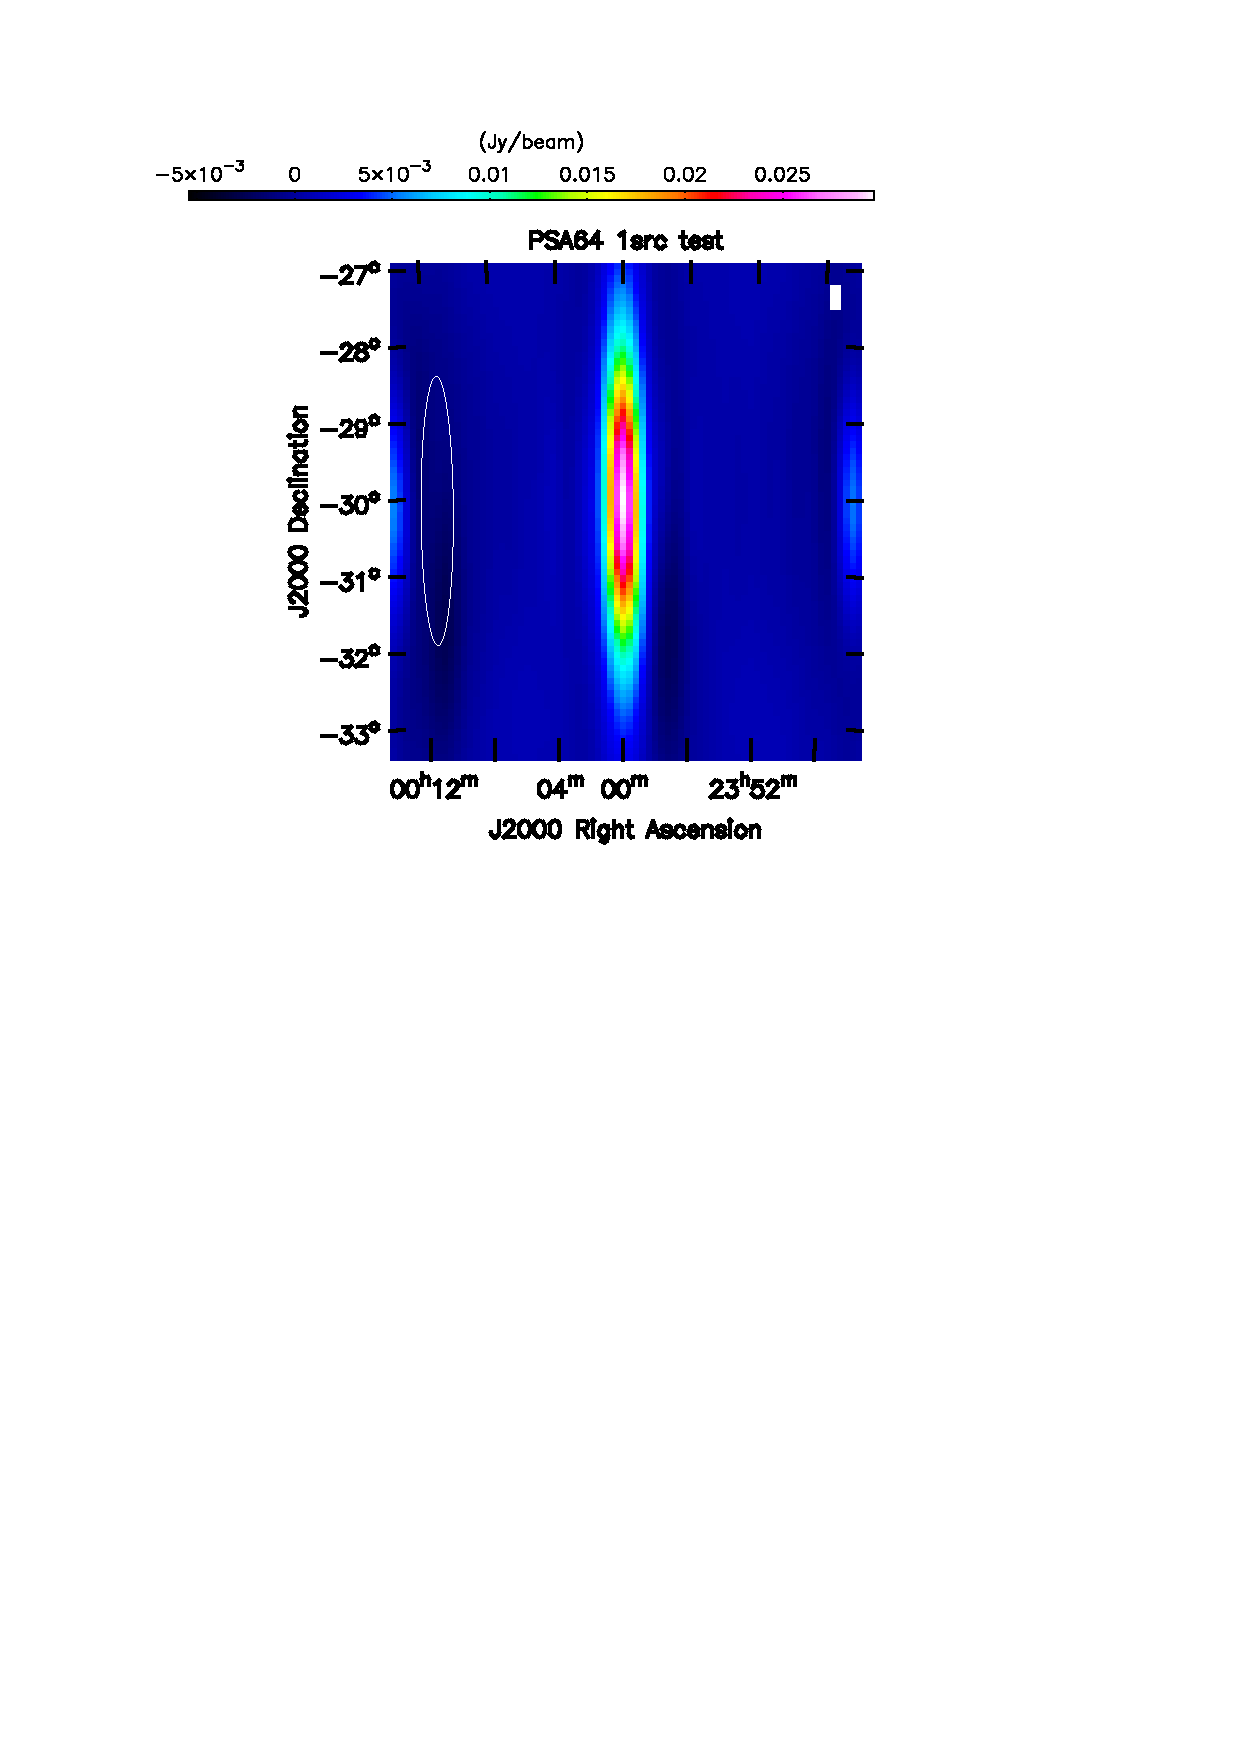
\includegraphics[width=.45\textwidth]{psa64_1src_test.png}
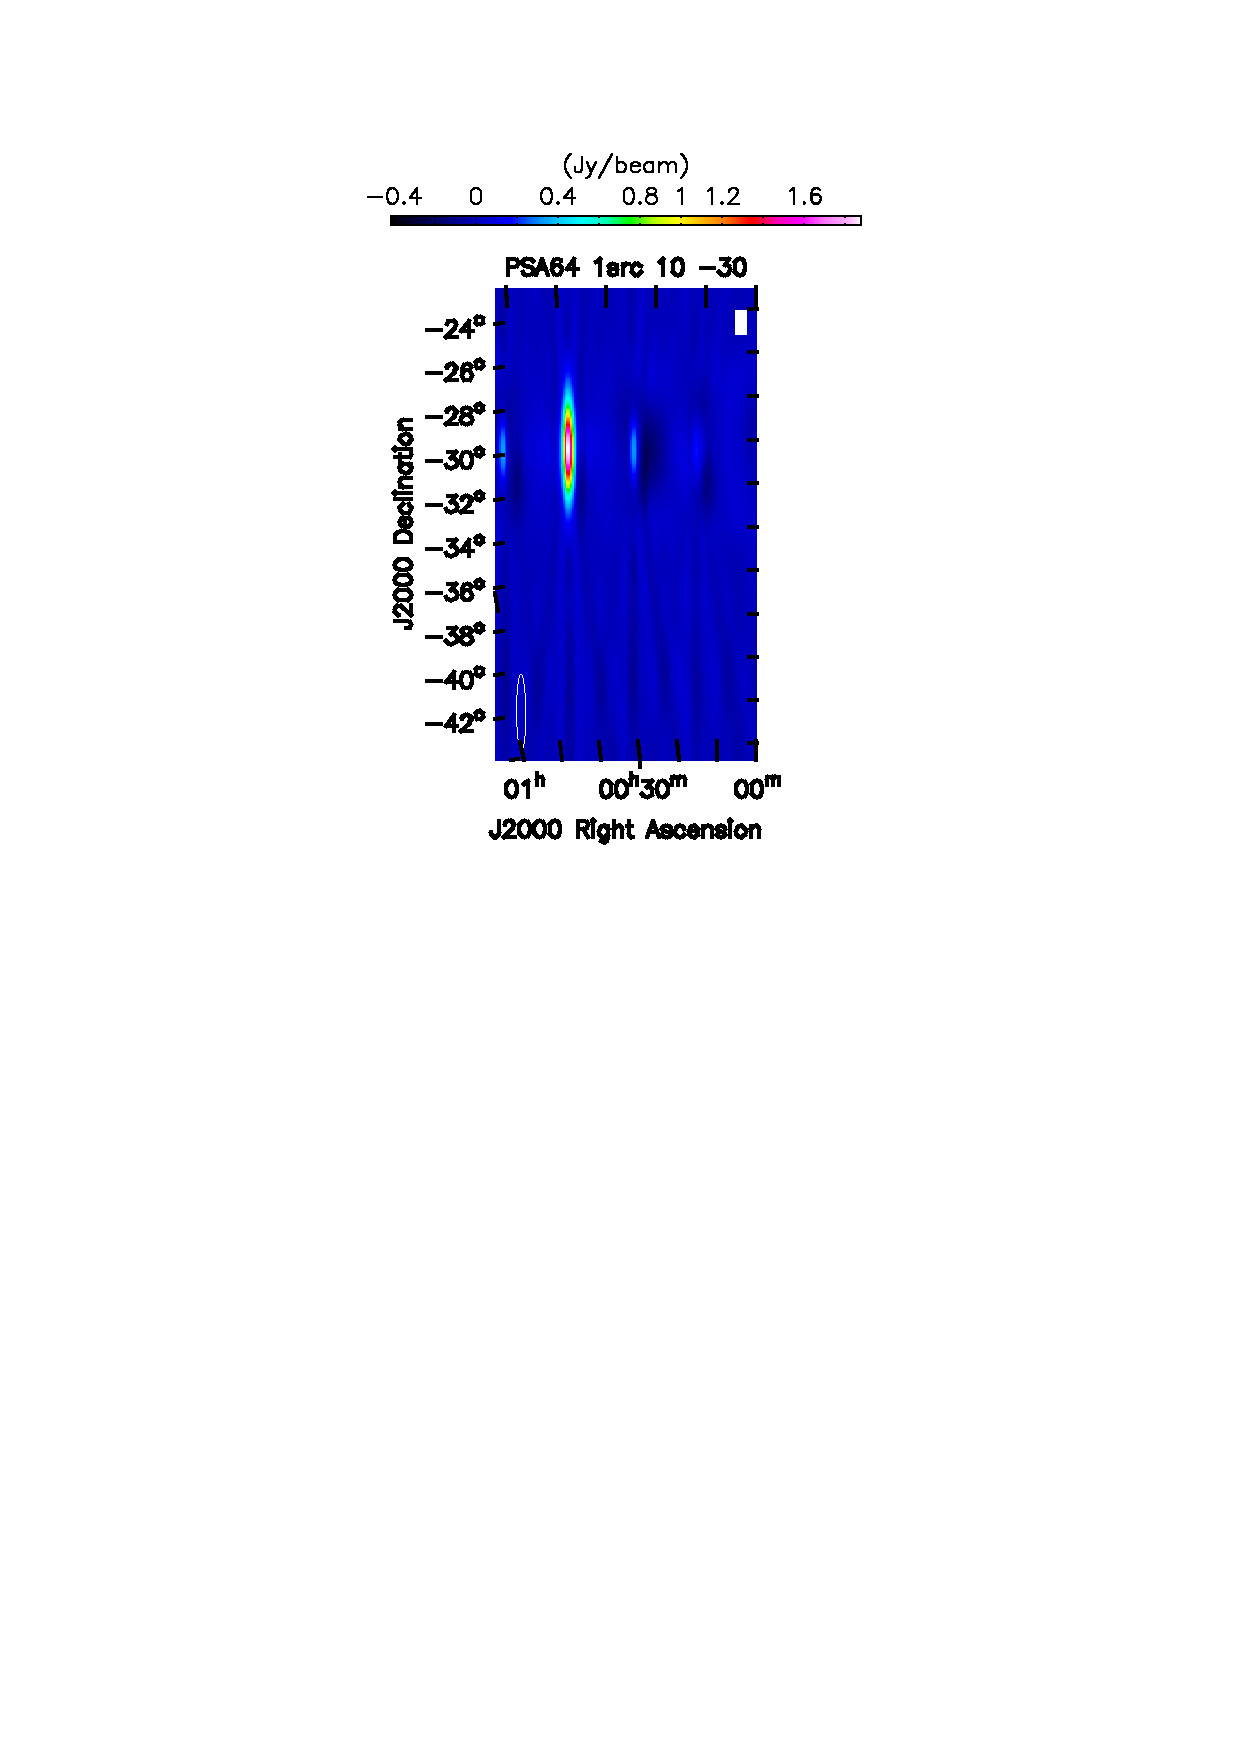
\includegraphics[width=.45\textwidth]{psa64_1src_10_-30.png}
\caption{Two test cases orientations of a single 500Jy point source. Left source position (0,-30\degree). Right source position (10\degree ,-30\degree)\label{fig:psa64_1src}}
\end{figure}
\section{Single Point Source Tests}{
Using a custom point source foreground model, I conduct tests of the imaging capabilities and configuration of PAPER-64 to verify the placement of sources on the sky.

The first tests use a 500Jy point source located at ra,dec (0,-30\degree) and (10,-30\degree). I use a multi-frequency synthesis to reconstruct these images using the built in CLEAN algorithm in CASA. The sidelobs in the PSF account for the "echoes" of the source seen in regular intervals.

The recovery of the point source at the desired sky positions with a PSF whose primary beam has a FWHM of 34 arcmins in the eastern direction and 3.8deg in the northern direction. These agree with the predictions for the PSF using the small angle approximation of the interference width $FWHM\sim \frac{\lambda}{D}$ where D is the baseline length.

}

\section{3 Point Source Test}{
The point source tests continue with a 3 source test pattern are described in \autoref{tab:3src}. I use this test to verify the location and possible parity flipping of the simulations.

\begin{table}[h]
\centering
\begin{tabular}{c c c}
RA & DEC & Flux (Jy) \\
\hline
0.0 & -26.701 &   1000.0  \\
5.0 & -41.701 & 100.0     \\
-20.0 & -5.701 &  50.0 
\end{tabular}
\caption{Position and sky Temperature of the 3 point sources used in test \label{tab:3src}}
\end{table}
The resulting image is display in \autoref{fig:psa64_3src}. The three point sources in \autoref{tab:3src} can be observed in the image accompanied by large side-lobe projections of the source at (-20\degree ,-5.701\degree). The presence of the sources at the desired locations verify the positioning of sources and parity used in the PRISim simulations.


\begin{figure}[h!]
\centering
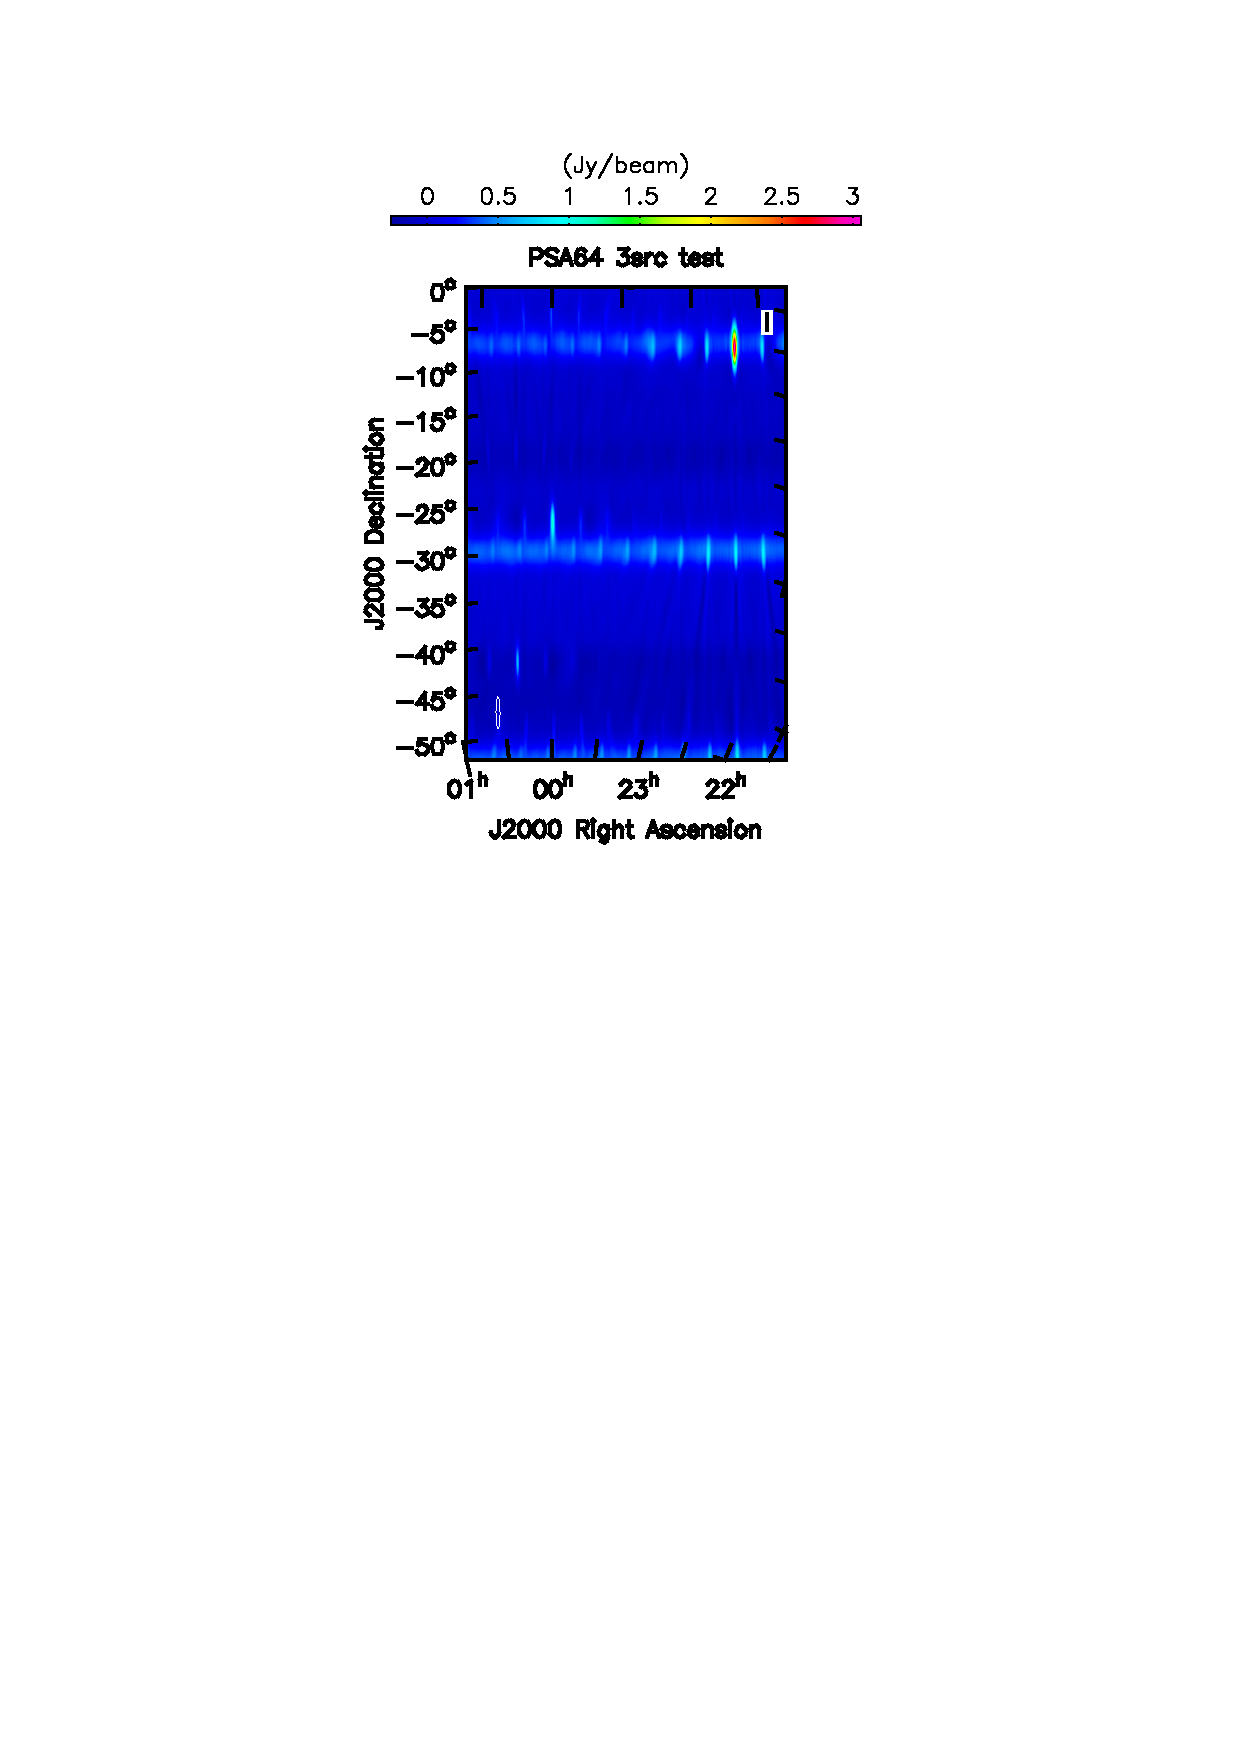
\includegraphics[width=.6\textwidth]{psa64_3src_test.png}
\caption{The 3 point source test configuration described in \autoref{tab:3src}. The large band near -30\degree Declination is a side-lobe projection of the source located at (-20\degree ,-5.701\degree) \label{fig:psa64_3src}}
\end{figure}

}

\section{Compact Sky Model}{
With confidence in the positioning, rotation, and parity of the simulations, I expand simulations to include a compact sky model composed of the NVSS and SUMSS point source catalogs without the test sources used above.

This simulation is conducted using both PAPER 64 and PAPER 128 telescopes and showing in \autoref{fig:paper_csm}. The increase in spatial resolution between the two deployments is apparent in the decreased source confusion; the confusion limit is still high compared to imaging arrays.

\begin{figure}[t]
\centering
%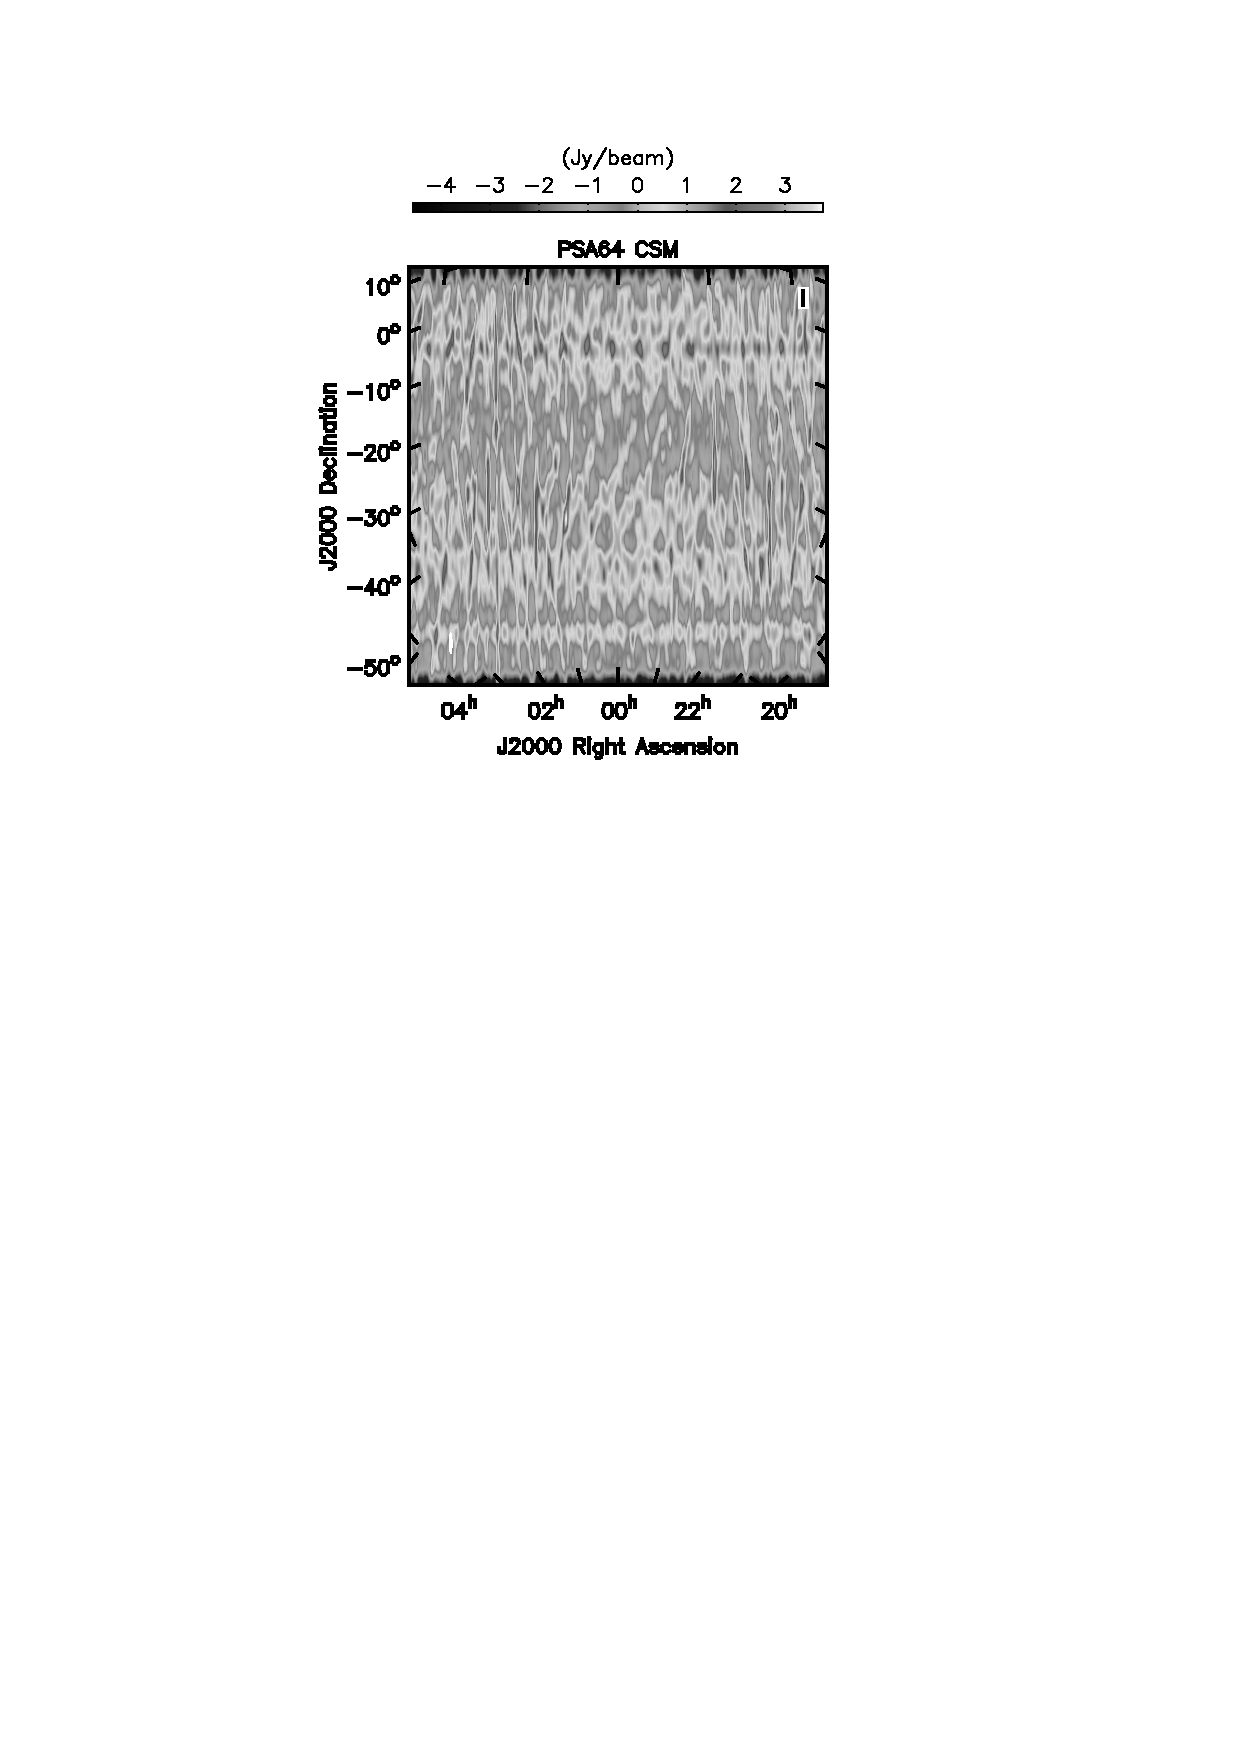
\includegraphics[width=.49\textwidth]{psa64_csm.png}
%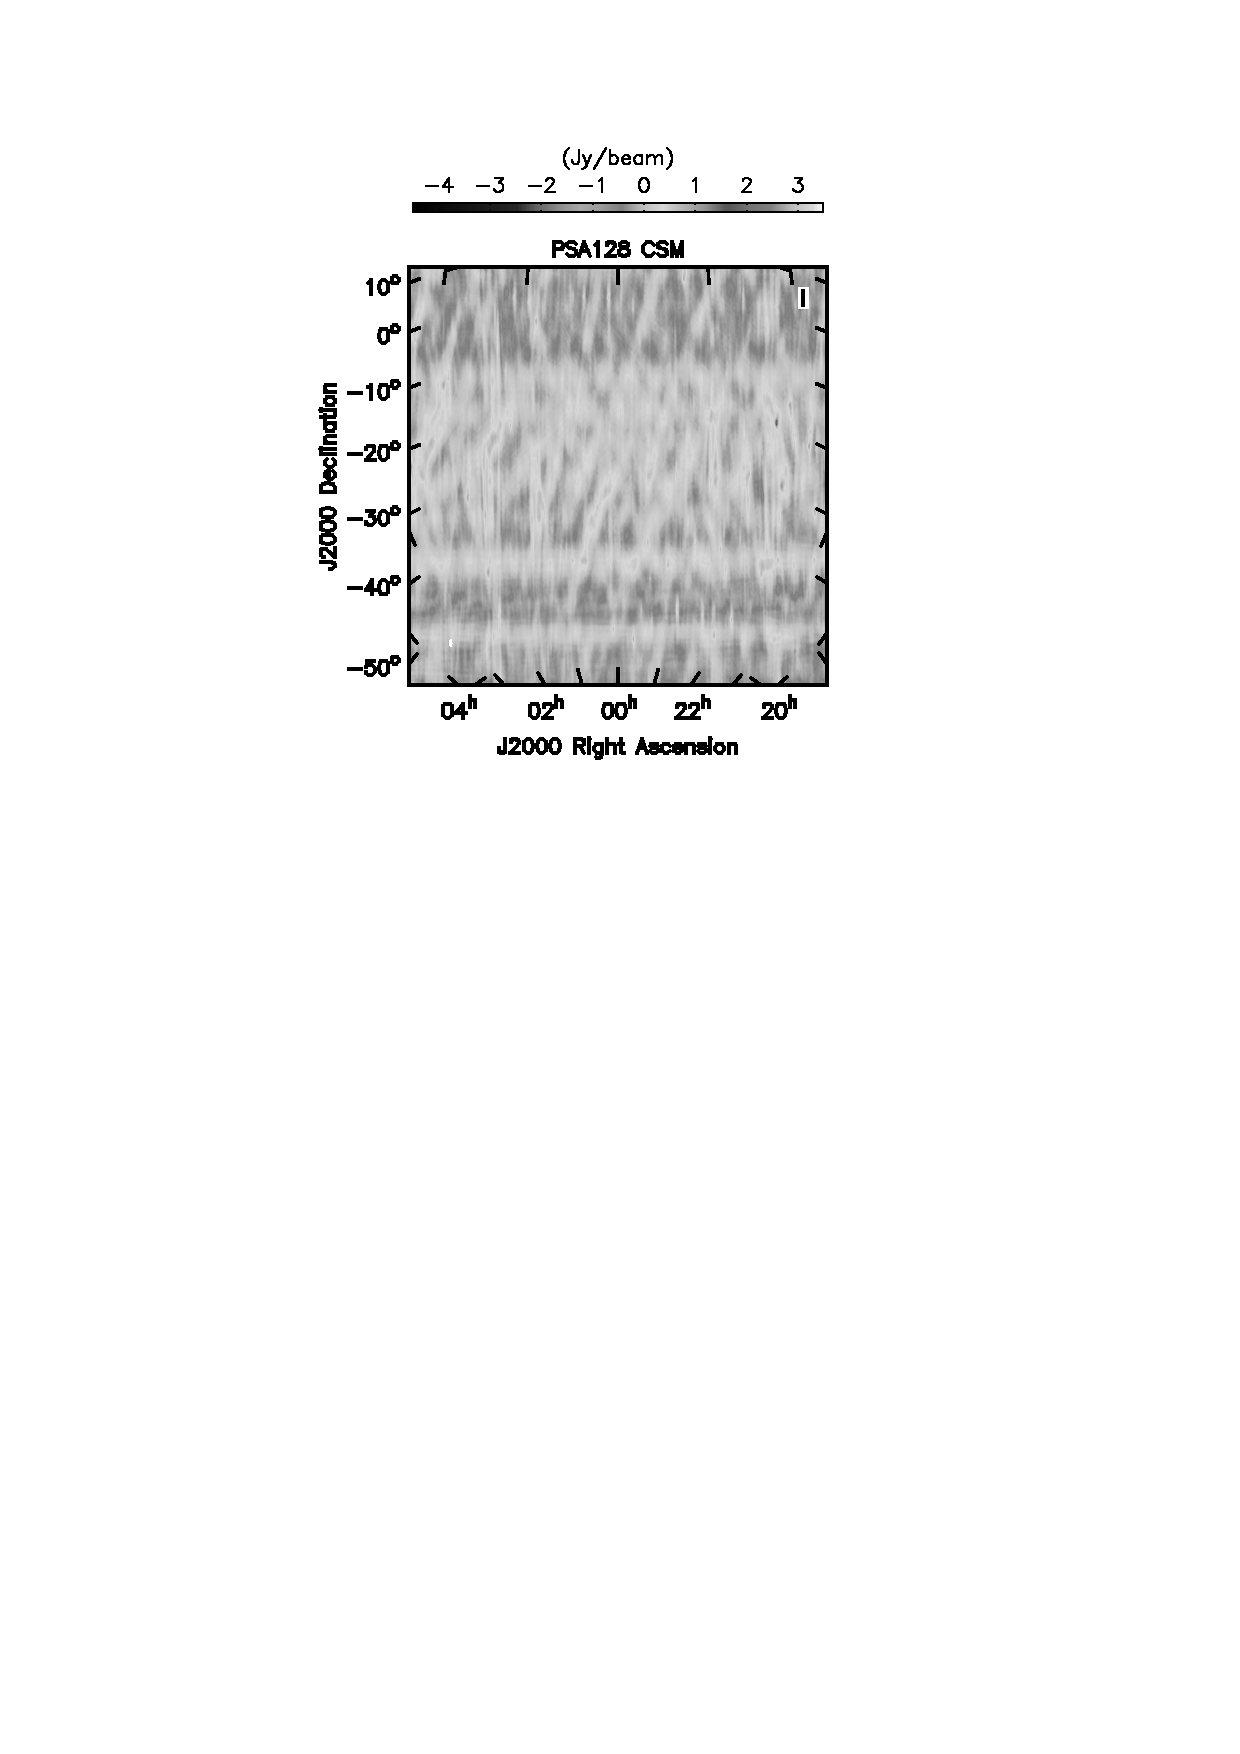
\includegraphics[width=.49\textwidth]{psa128_csm.png}
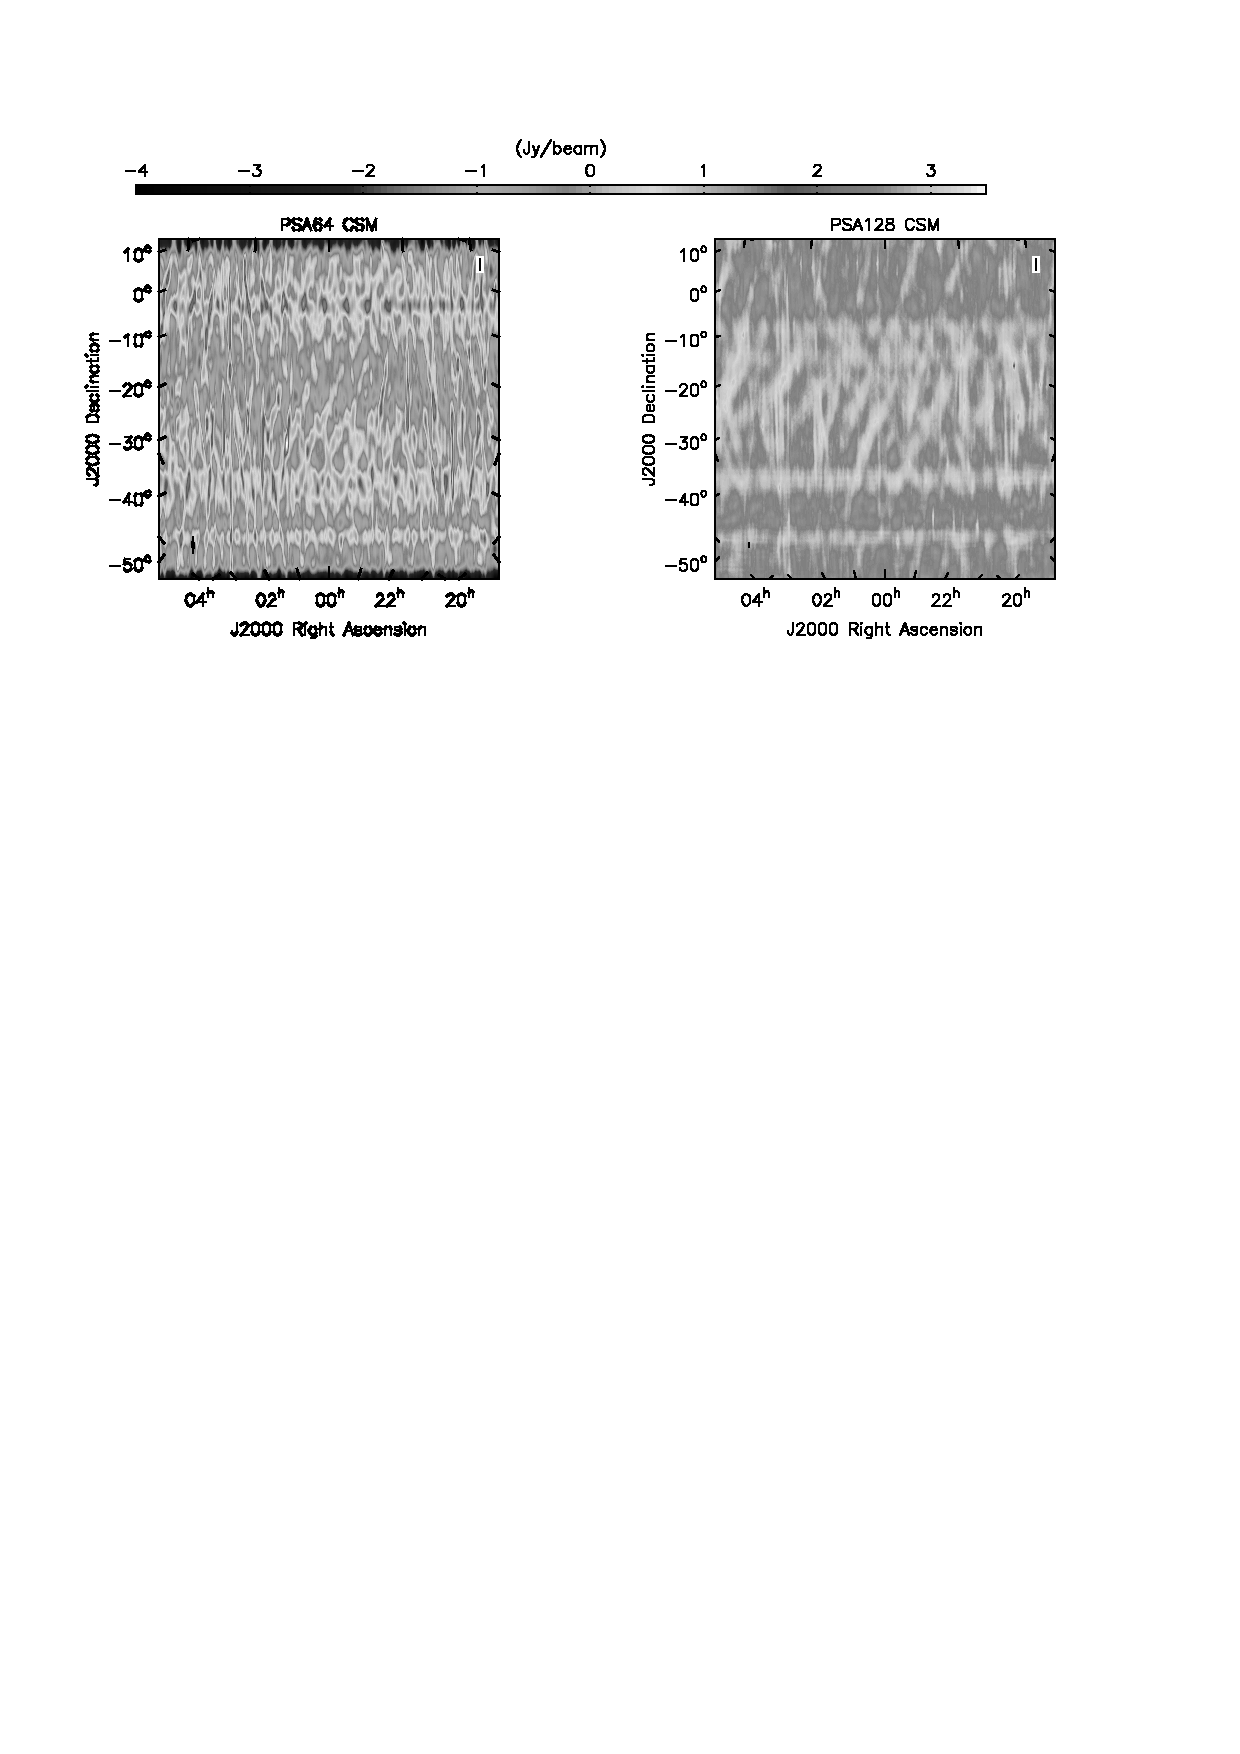
\includegraphics[width=.8\textwidth]{paper_csm_compare.png}
\caption{\label{fig:paper_csm} A full sky compact sources simulation made from NVSS and SUMSS catalogs imaged on Left: PAPER 64 and Right: PAPER 128. Side-lobe power is significantly decreased in the 128 antenna deployment.}
\end{figure}

}

\begin{table}[p]
\centering
\begin{tabular}{c c c}
\hline
Array &Simulation  & prisim\_runs git hash \\ \hline \hline
PSA64 & Point Sources & 1246307095895293cdcf2aae035ac931b751654b \\
PSA64 & CSM & 390717fc94254494c72603acda6dbab13df09621 \\
PSA128 & CSM & 63df1dd0bd3bbe213878588b6143f6d612aceb49 \\ \hline \hline
\multicolumn{3}{c}{PRISim git hash} \\
\multicolumn{3}{c}{390717fc94254494c72603acda6dbab13df09621}
\end{tabular}
\caption{\label{tab:githash} The git hashes used for the prism\_runs configuration yaml files and the PRISim source code}
\end{table}


\end{document}